% presentation.tex — ThetaSwap Beamer Slide Deck
% Adverse Competition Oracle: Problem, Evidence, Solution, Demo, Roadmap
% Frames 1-6 (Title + Problem + Evidence) — Plan 04-01
% Frames 7-10 (Solution + Demo + Roadmap) — Plan 04-02

\documentclass[aspectratio=169]{beamer}

% ── Theme and Colors ─────────────────────────────────────────────────────────
\usetheme{Madrid}
\definecolor{thetablue}{RGB}{20,40,80}

% Override beamer colors for dark blue + white
\setbeamercolor{structure}{fg=thetablue}
\setbeamercolor{palette primary}{bg=thetablue,fg=white}
\setbeamercolor{palette secondary}{bg=thetablue!80,fg=white}
\setbeamercolor{palette tertiary}{bg=thetablue!60,fg=white}
\setbeamercolor{palette quaternary}{bg=thetablue,fg=white}
\setbeamercolor{frametitle}{bg=thetablue,fg=white}
\setbeamercolor{title}{fg=white,bg=thetablue}
\setbeamercolor{subtitle}{fg=white}
\setbeamercolor{author}{fg=white}
\setbeamercolor{date}{fg=white}
\setbeamercolor{institute}{fg=white}
\setbeamercolor{block title}{bg=thetablue,fg=white}
\setbeamercolor{block body}{bg=thetablue!5,fg=black}
\setbeamercolor{item}{fg=thetablue}
\setbeamercolor{normal text}{fg=black,bg=white}

% Remove navigation symbols and section navigation bar
\setbeamertemplate{navigation symbols}{}
\setbeamertemplate{headline}{}

% ── Packages ─────────────────────────────────────────────────────────────────
\usepackage{amsmath,amssymb}
\usepackage{booktabs}
\usepackage{graphicx}
\usepackage{xcolor}
\usepackage{natbib}
\bibliographystyle{abbrvnat}

% ── Macros (from preamble.tex — standalone, no \input) ──────────────────────
\newcommand{\AT}{A_T}
\newcommand{\ThetaSum}{\Theta}
\newcommand{\PosCount}{N}
\newcommand{\ATnull}{A_T^{1/\PosCount}}
\newcommand{\DeltaPlus}{\Delta^{+}}
\newcommand{\DeltaStar}{\Delta^{*}}
\newcommand{\thetapos}{\theta}
\newcommand{\blocklife}{\ell}

% ── Title Metadata ───────────────────────────────────────────────────────────
\title{ThetaSwap: Adverse Competition Oracle}
\author{ThetaSwap}
\date{\today}

% ══════════════════════════════════════════════════════════════════════════════
\begin{document}

% ── Frame 1: Title ───────────────────────────────────────────────────────────
\begin{frame}[plain]
\titlepage
\end{frame}

% ── Frame 2: Problem — The Risk Nobody Hedges ────────────────────────────────
\begin{frame}{The Risk Nobody Hedges}

In a symmetric equilibrium, each of $\PosCount$ LPs earns $1/\PosCount$ of
fees \citep{macrapis2024permissionless}. In practice, sophisticated actors
concentrate fee revenue away from passive participants.
This is \textbf{adverse competition} --- a distinct, unhedged risk.

\bigskip

\begin{itemize}
  \item \textbf{Impermanent loss (IL)} --- price divergence between pool assets.
    Variance perpetuals perfectly hedge IL
    \citep{fukasawa2023weighted}; Panoptic deploys this on-chain.

  \item \textbf{Loss-versus-rebalancing (LVR)} --- adverse selection cost from
    informed traders. MEV-aware products address LVR.

  \item \textbf{Fee concentration risk} --- the \emph{competition structure}
    among LPs for fee revenue, captured by the FLAIR metric
    \citep{milionis2024flair}.
    \textcolor{red}{\textbf{Nothing hedges this today.}}
\end{itemize}

\end{frame}

% ── Frame 3: Research Question & Methodology ─────────────────────────────────
\begin{frame}{Research Question}

\textbf{Is there empirical demand for a hedging instrument against adverse
competition? If so, how much are LPs willing to pay?}

\bigskip

\begin{block}{Data}
ETH/USDC 30bps pool (Uniswap V3 mainnet) \\
41 days $\cdot$ 600 positions $\cdot$ 3,365 position-day observations $\cdot$ 597 exits
\end{block}

\medskip

\textbf{Methodology:}
\begin{itemize}
  \item Compute fee concentration index $\AT$ and competitive null $\ATnull$
    per day from on-chain Collect/Burn/Mint events
  \item Define treatment variable: deviation $\Delta = \AT - \ATnull$
  \item Estimate exit hazard as a function of $\Delta$ with IL and position
    age controls, clustered standard errors
  \item Real $\AT$ exceeds the null by $2.65\times$ on average; 63\% of days
    show $\DeltaPlus > 0$
\end{itemize}

\end{frame}

% ── Frame 4: Evidence — Model Specification ──────────────────────────────────
\begin{frame}{Model Specification}

\textbf{Why quadratic?} A linear model yields $\beta_1 < 0$ (shelter effect)
--- concentration correlates with volume, masking the exit signal. Dose-response
analysis reveals non-monotonicity: exits peak at moderate $\Delta$, then drop.
A quadratic term captures both regimes in one specification.

\medskip

\begin{center}
\boxed{
  P(\text{exit}_{i,t}) = \sigma\!\bigl(
    \beta_0
    + \beta_1 \underbrace{\Delta_{t-\ell}}_{\text{shelter}}
    + \beta_2 \underbrace{\Delta_{t-\ell}^2}_{\text{Capponi exit}}
    + \beta_3 \,\text{IL}_t
    + \beta_4 \log(\text{age}_{i,t})
  \bigr)
}
\end{center}

\medskip

\begin{itemize}
  \item $\Delta = \AT - \ATnull$: deviation from competitive null
  \item $\text{IL}_t$: impermanent loss control (orthogonality test)
  \item $\log(\text{age})$: duration dependence
  \item \textbf{Expected:} $\beta_1 < 0$ (shelter), $\beta_2 > 0$ (exit above threshold)
\end{itemize}

\end{frame}

% ── Frame 5: Evidence — Empirical Results ────────────────────────────────────
\begin{frame}{Empirical Results}

\begin{center}
\begin{tabular}{@{}cccccl@{}}
\toprule
Lag & $\hat{\beta}_1$ (linear) & $p$ & $\hat{\beta}_2$ (quadratic) & $p$ & Turning point \\
\midrule
\textbf{1} & $\mathbf{-23.18}$ & $\mathbf{0.012}$ & $\mathbf{+129.20}$ & $\mathbf{0.030}$ & $\mathbf{0.090}$ \\
\textit{2} & \textit{$-43.42$} & \textit{0.016} & \textit{$+226.92$} & \textit{0.065} & \textit{0.096} \\
\textbf{3} & $\mathbf{-32.44}$ & $\mathbf{0.001}$ & $\mathbf{+205.34}$ & $\mathbf{0.004}$ & $\mathbf{0.079}$ \\
\bottomrule
\end{tabular}
\end{center}

\bigskip

\begin{itemize}
  \item \textbf{Lags 1 and 3}: both coefficients significant at 5\%
  \item \textbf{Lag 2}: linear significant, quadratic marginal ($p = 0.065$)
  \item Signal \textbf{dissipates at lags 5--7} --- LPs react to recent shocks
\end{itemize}

\end{frame}

% ── Frame 6: Evidence — The Inverted-U ───────────────────────────────────────
\begin{frame}{The Inverted-U}

\begin{columns}[T]

\begin{column}{0.50\textwidth}
\textbf{Two regimes:}

\medskip

\begin{enumerate}
  \item \textbf{Shelter} ($\Delta < 0.09$) \\
    Mild concentration is protective --- elevated volume benefits all LPs.

  \medskip

  \item \textbf{Capponi} ($\Delta > 0.09$) \\
    Extreme concentration drives exits --- passive LP fee rate drops below
    exit threshold.
\end{enumerate}

\bigskip

Turning point:
\[
  \DeltaStar = \frac{-\beta_1}{2\beta_2} = \frac{23.18}{2 \times 129.20} = 0.090
\]

At $\Delta = 0.15$: marginal effect $= 2.27$ \\
{\small Each 0.01 increase raises exit probability by ${\sim}2.3$ pp}
\end{column}

\begin{column}{0.45\textwidth}
\begin{center}
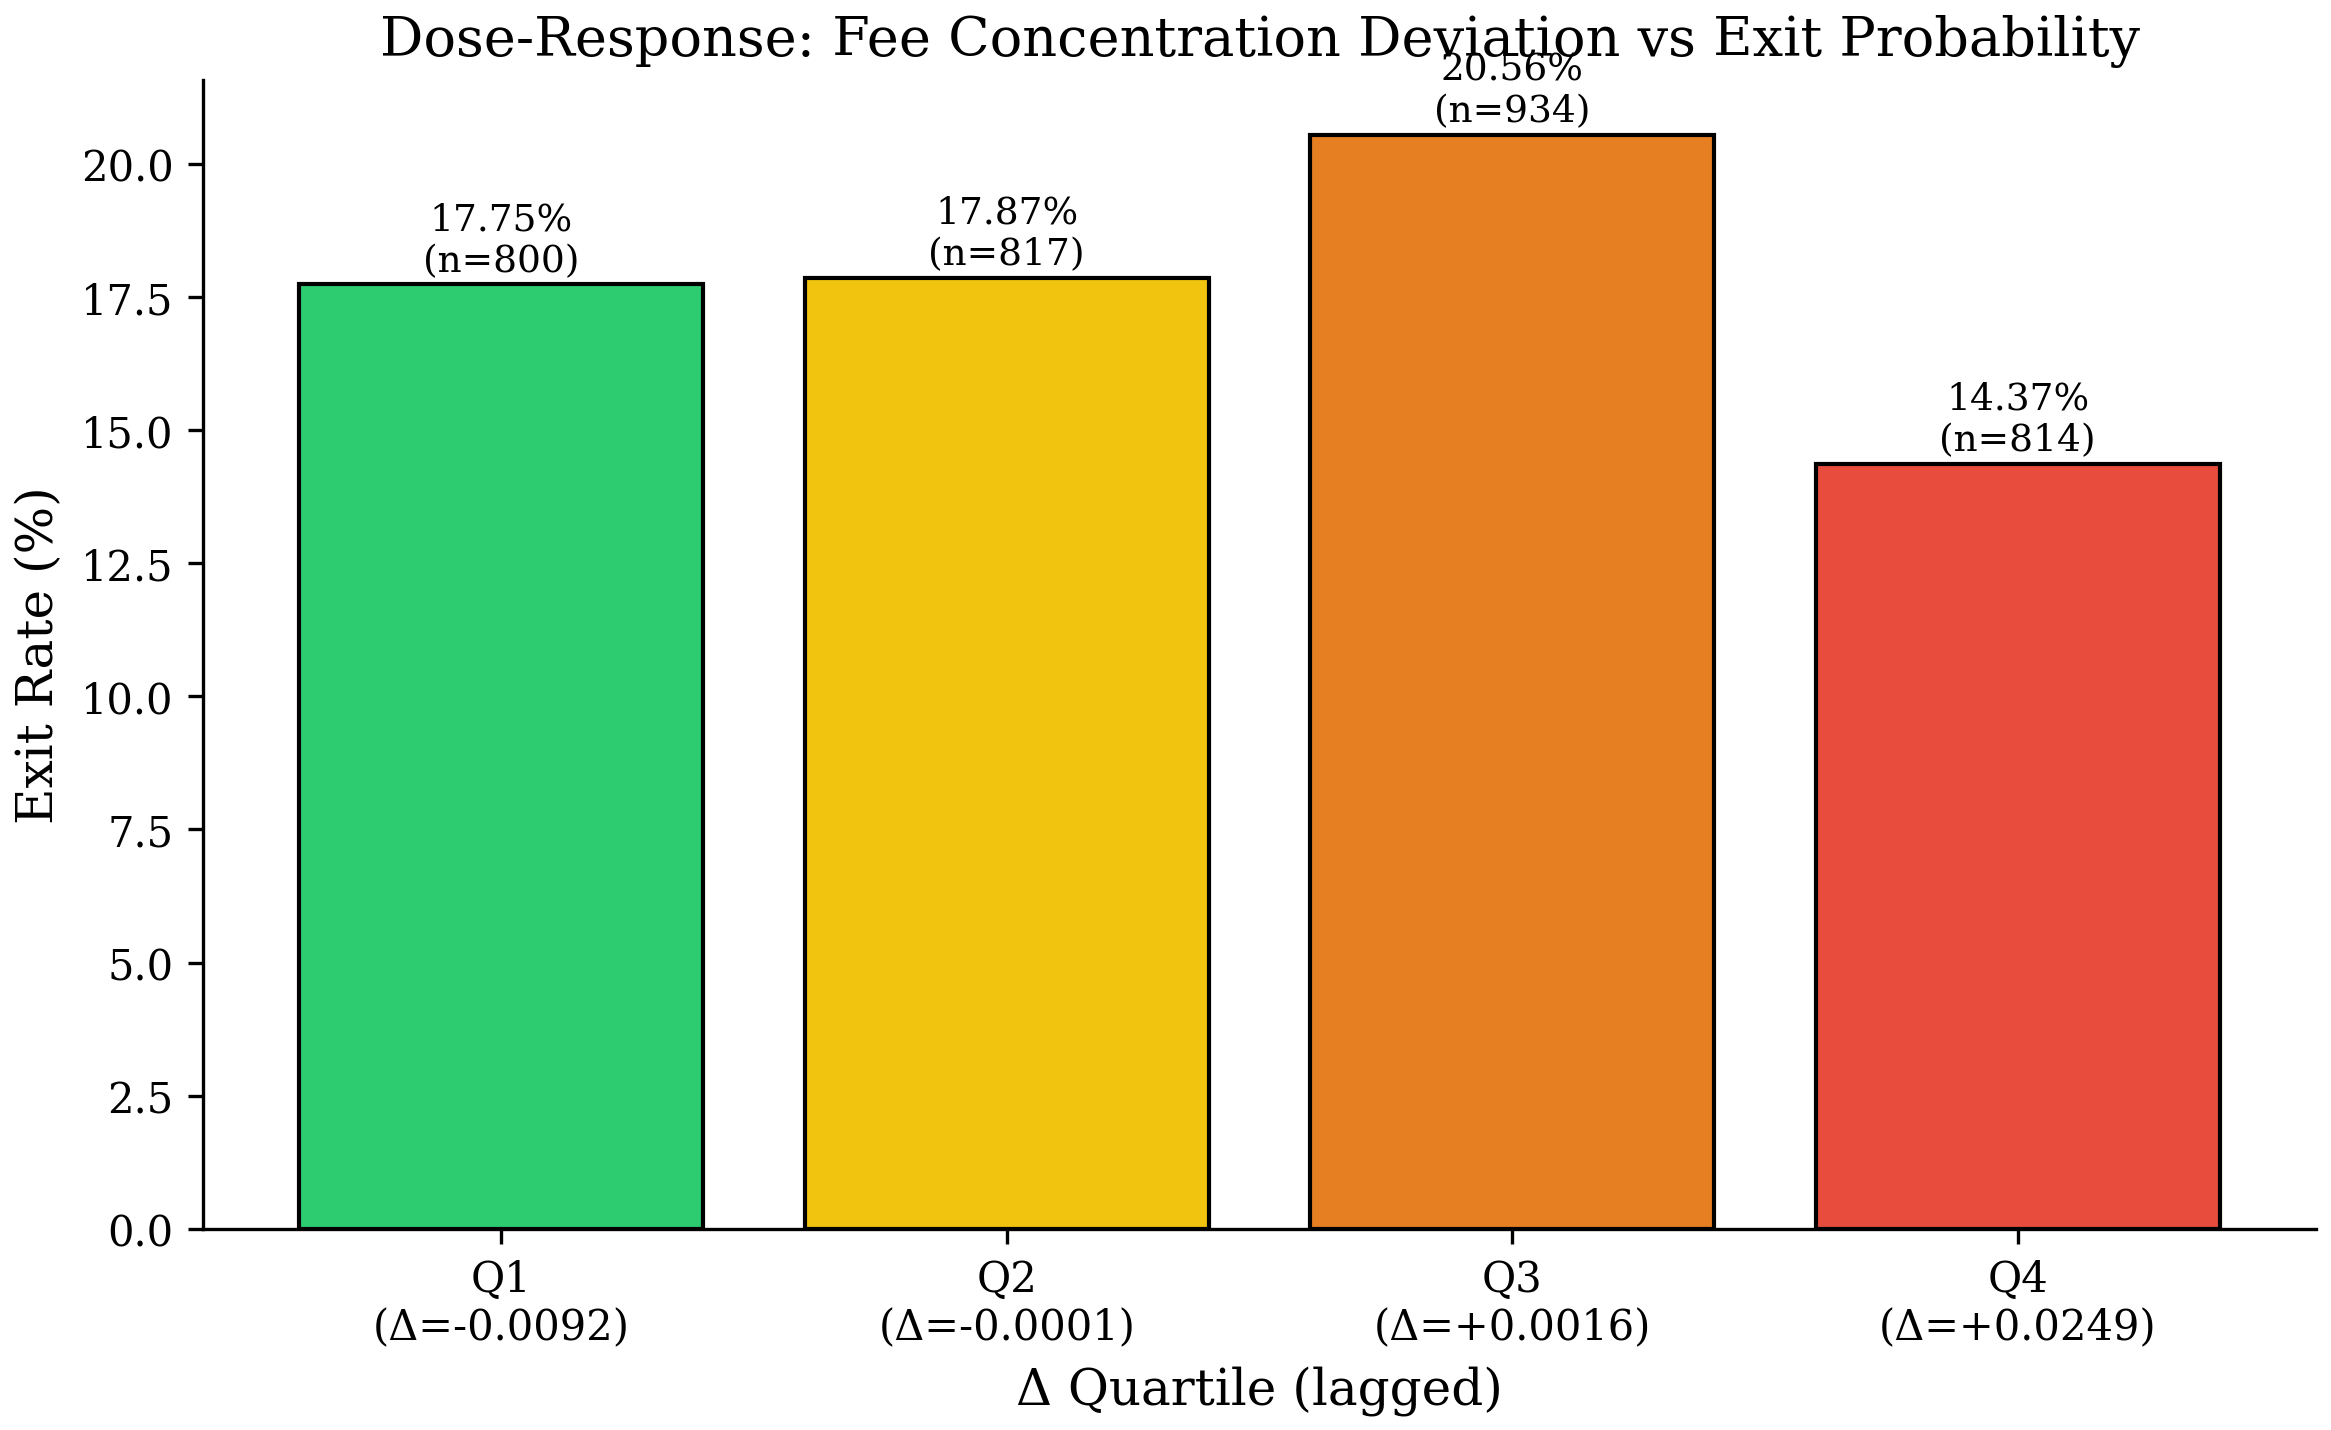
\includegraphics[width=\textwidth]{../figures/dose-response.png}
\end{center}
\end{column}

\end{columns}

\end{frame}

% ── Frame 7: Solution — Architecture ─────────────────────────────────────────
\begin{frame}{Architecture}

\begin{center}
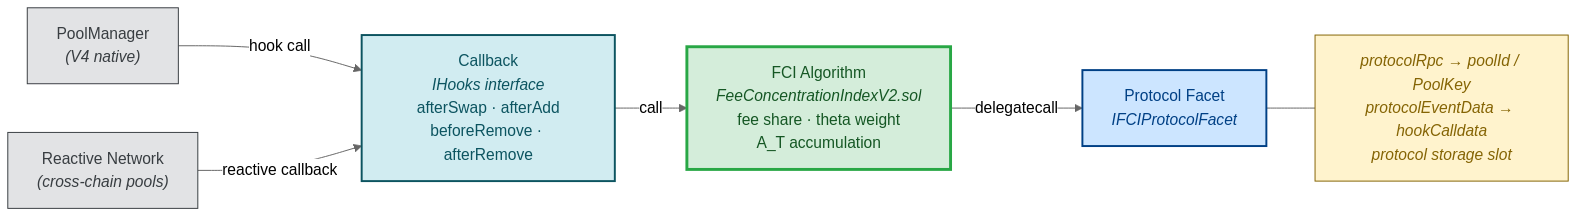
\includegraphics[width=\textwidth]{../../docs/diagrams/context-diagram.png}
\end{center}

\medskip

FCI Hook at center --- protocol adapters (V3, V4) feed swap/mint/burn events,
Reactive Network bridges metrics cross-chain, Vault + CFMM settle downstream.

\end{frame}

% ── Frame 8: Solution — Cross-Protocol Modularity ────────────────────────────
\begin{frame}{Cross-Protocol Modularity}

\begin{center}
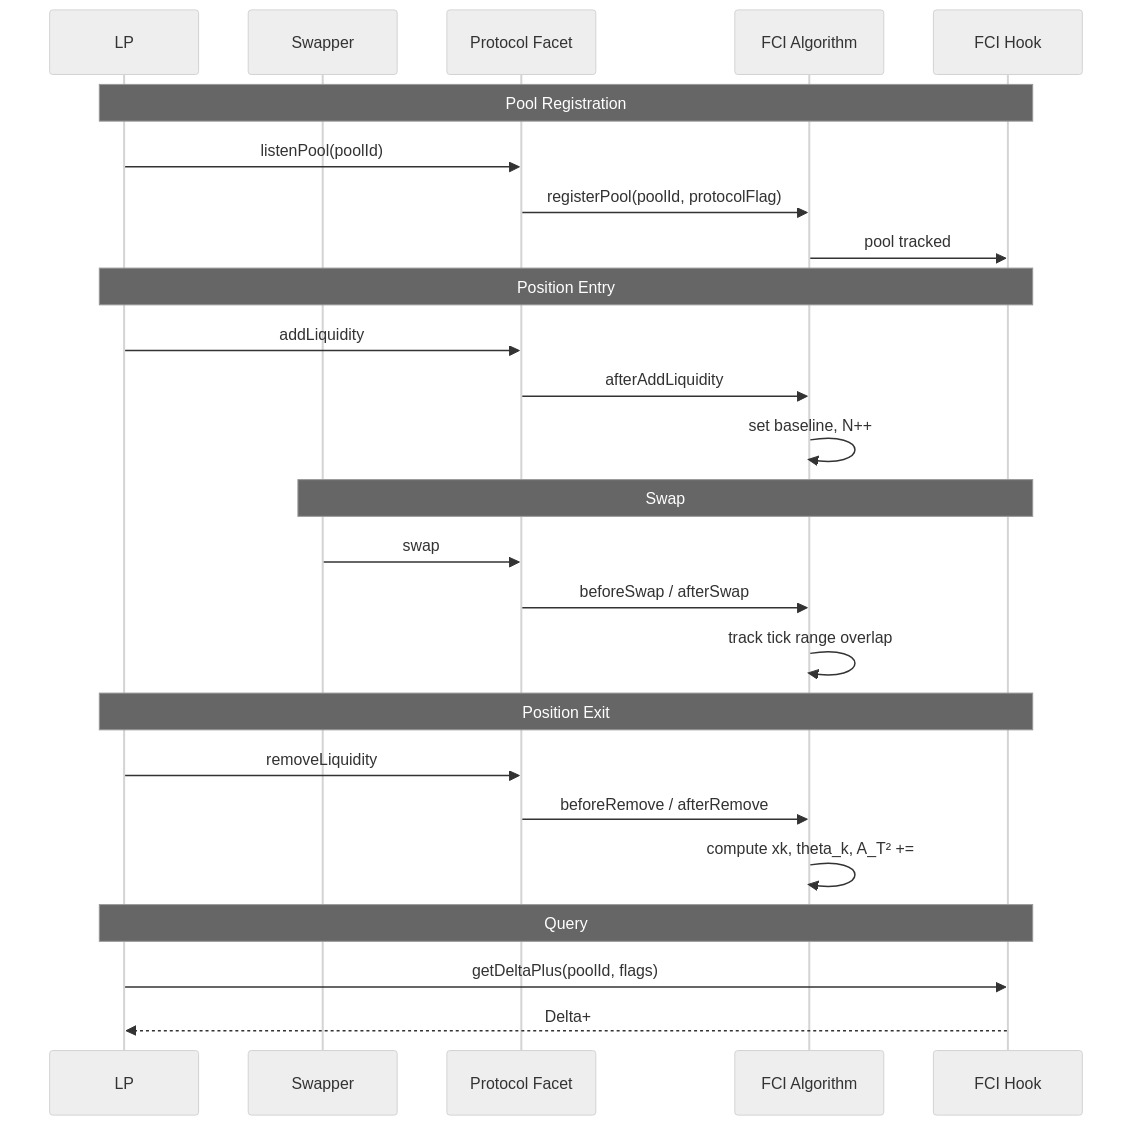
\includegraphics[height=0.75\textheight]{../../docs/diagrams/sequence-diagram.png}
\end{center}

\medskip

\texttt{listenPool()} $\to$ swap/mint/burn events $\to$ metric update $\to$
$\DeltaPlus$ derivation. \\
Same FCI oracle, multiple protocol adapters, reactive network bridges events
cross-chain.

\end{frame}

% ── Frame 9: Demo — Live Demo ────────────────────────────────────────────────
\begin{frame}{Live Demo}

\begin{block}{Run the integration test}
\small
\texttt{forge test --match-path} \\
\texttt{"test/fee-concentration-index-v2/protocols/uniswapV4/} \\
\texttt{NativeV4FeeConcentrationIndex.integration.t.sol" -vv}
\end{block}

\bigskip

\textbf{What to observe:}

\begin{enumerate}
  \item Swap updates $\AT$ --- fee concentration index tracks each trade
  \item Mint increments $\PosCount$ --- new positions enter the pool
  \item Burn triggers $\DeltaPlus$ derivation --- exit computes concentration
    deviation
  \item All metrics computed on-chain in a single V4 hook callback
\end{enumerate}

\end{frame}

% ── Frame 10: Roadmap — What's Next ──────────────────────────────────────────
\begin{frame}{What's Next}

\begin{columns}[T]

\begin{column}{0.48\textwidth}
\textbf{Built}

\begin{itemize}
  \item FCI oracle live on Uniswap V4
  \item Reactive adapter bridging V3 events cross-chain
  \item Backtest validation: 18.8\% of positions better off hedged,
    +\$23 mean hedge value
\end{itemize}
\end{column}

\begin{column}{0.48\textwidth}
\textbf{Next}

\begin{itemize}
  \item Linearized power-squared CFMM (trading function complete in spec)
  \item Vault settlement mechanism
\end{itemize}
\end{column}

\end{columns}

\bigskip

\begin{center}
\textit{The mathematical specification is complete, the oracle tracks metrics
across protocols, and the next milestone delivers the full insurance product.}
\end{center}

\end{frame}

% ── References ────────────────────────────────────────────────────────────────
\begin{frame}[allowframebreaks]{References}
\footnotesize
\bibliography{../model/references}
\end{frame}

% ══════════════════════════════════════════════════════════════════════════════
\end{document}
